%% Appendix sections
%% Content migrated from the journal-style main text back into appendix.


\section{Extended Related Work}
\label{app:extended_related_work}

This section provides an extended discussion of the related work summarized in Section~\ref{sec:related_work}, offering additional technical details on representative methods in each line of research.

\subsection{Early and Statistical Methods}
Early tabular data synthesis methods relied on statistical techniques. SMOTE~\cite{chawla2002smote} generates synthetic minority-class samples by interpolating between nearest neighbors in feature space, addressing class imbalance but limited to local linear combinations. Copula-based methods~\cite{xue2000multivariate} model the joint distribution by separately estimating marginal distributions and their dependency structure through copula functions, providing a principled statistical framework but struggling to capture complex, non-linear inter-feature relationships. These foundational approaches established the core objectives of tabular synthesis---realistic sample generation with dependency preservation---but their limited expressiveness motivated the shift toward deep generative models.

\subsection{Deep Generative Models for Tabular Data}
Deep generative models learn the data distribution through expressive neural architectures. TVAE~\cite{patki2016synthetic} adapts the Variational Autoencoder framework to mixed-type tabular data by applying mode-specific normalization to continuous columns. CTGAN~\cite{xu2019modeling} introduces a conditional GAN with a training-by-sampling strategy that addresses the imbalanced categorical distributions common in tabular datasets. Normalizing Flow-based methods~\cite{papamakarios2021normalizing} learn invertible transformations between a simple base distribution and the data distribution, offering exact likelihood computation. More recently, diffusion-based approaches have achieved strong results: TabDDPM~\cite{kotelnikov2023tabddpm} applies denoising diffusion probabilistic models to tabular data with separate handling of numerical and categorical features, while TabSyn~\cite{tabsyn} first encodes mixed-type tabular data into a continuous latent space via a VAE and then applies score-based diffusion within that space, improving inter-column relation fidelity while reducing inference steps. Despite these advances, all DGM-based approaches learn feature dependencies only as a byproduct of distribution fitting, offering limited interpretability or explicit control over the dependency structure during generation.

\subsection{Structure-Aware Generative Methods}
Structure-aware methods explicitly incorporate graphical models of feature dependencies into the generative process. Bayesian Network-based generators~\cite{ankan2015pgmpy} learn a directed acyclic graph over features and sample from the resulting factorized joint distribution. PrivBayes~\cite{zhang2017privbayes} extends this framework with differential privacy guarantees by injecting calibrated noise into the learned conditional distributions, enabling privacy-preserving synthesis. Among deep-learning approaches, DECAF~\cite{van2021decaf} leverages a user-specified or learned causal graph to achieve fairness-aware generation by intervening on sensitive attributes, while GOGGLE~\cite{liu2023goggle} employs a graph-based VAE that jointly learns the dependency structure and the generative model in an end-to-end differentiable manner. However, the quality of these methods is fundamentally tied to the accuracy of the underlying graph, which degrades substantially under limited-sample settings where conditional independence tests lack statistical power and score-based search becomes prone to local optima. More recently, SPADA~\cite{yang2025doubling} employs an LLM to annotate sparse feature dependencies as a directed graph, then synthesizes data by traversing the graph with kernel density estimation or conditional normalizing flows, bypassing LLM-based generation entirely to achieve substantial sampling speedups.

\subsection{LLM-Based Tabular Generation: Extended Discussion}
Beyond the prompt-based and structure-aware LLM methods discussed in the main text, several fine-tuning approaches have been proposed. GReaT~\cite{borisov2023language} serializes each table row as a natural-language sentence with randomized column ordering and fine-tunes a pre-trained GPT-2 model for autoregressive row generation. TAPTAP~\cite{zhang2023generative} introduces a table pre-training stage that exposes the LLM to diverse tabular datasets before task-specific fine-tuning, improving generalization across domains. AIGT~\cite{zhang2025aigt} further augments the fine-tuning paradigm with attribute-level instruction tuning, enabling the model to follow explicit generation directives for individual columns. While these fine-tuning methods can achieve high fidelity when sufficient training data is available, they incur substantial computational costs and their performance degrades markedly in low-data regimes ($n \le 100$) where the limited training set is insufficient for effective parameter adaptation.

\section{Structure Learning Background}
\label{app:structure_learning_background}

\subsection{Conventional Structure Learning}
Conventional approaches to dependency structure discovery primarily fall into two categories: constraint-based and score-based methods. Constraint-based methods, such as the Peter--Clark (PC) algorithm~\cite{spirtes2000causation} and the Fast Causal Inference (FCI) algorithm~\cite{spirtes1995causal}, utilize conditional independence tests to iteratively prune edges from an initially fully connected graph. While PC assumes causal sufficiency (no hidden confounders), FCI is specifically designed to handle latent variables. In contrast, score-based methods optimize a global scoring criterion to identify the most suitable graph structure. A representative example is the Greedy Equivalence Search (GES)~\cite{chickering2002optimal}, which searches through equivalence classes to maximize a scoring function. However, both constraint-based and score-based approaches typically yield only Markov equivalence classes, thereby failing to distinguish between structurally distinct graphs that encode identical conditional independencies. To address this limitation, Functional Causal Models (FCMs) impose stronger assumptions regarding the data generation process. FCMs model effects explicitly as functions of direct causes combined with independent noise terms, enabling the identification of causal directions since independence between cause and noise typically breaks down when reversed~\cite{shimizu2006linear, hoyer2008nonlinear, zhang2009identifiability}. Recent advancements have generalized this approach, introducing conditions such as Generalized Independent Noise (GIN) to manage latent causal variables in linear, non-Gaussian settings~\cite{xie2020generalized}. However, the statistical power of these traditional algorithms heavily relies on a large number of samples, making them unreliable for structure discovery in the low-data regimes addressed by our work.

\subsection{LLM-based Structure Learning}
Leveraging Large Language Models (LLMs) for structure learning has recently emerged as a promising direction due to their inherent reasoning capabilities. Several paradigms have been proposed for integrating LLMs into structure discovery. Initially, methods focused on querying LLMs about pairwise causal relationships, showing strong accuracy in determining causal directions between variable pairs~\cite{kiciman2023causal}. To overcome the quadratic complexity inherent to pairwise approaches, more scalable methods employing breadth-first search (BFS) strategies have been introduced, reframing structure learning as a graph traversal task and significantly reducing the required number of queries to the LLM~\cite{jiralerspong2024efficient, zanna2025fairness}. A third paradigm enhances reliability by integrating an iterative supervision loop, in which traditional structure-learning algorithms propose initial graphs that are subsequently validated or corrected by LLMs. This method grounds LLM-generated structures in empirical evidence, thereby reducing hallucination risks~\cite{ban2023causal}. LLM-based structure discovery methods have demonstrated notable effectiveness across diverse domains, including medicine~\cite{naik2024applying, antonucci2023zero, arsenyan2024large}, economics~\cite{causal4financial}, and social sciences~\cite{manning2024automated}. Inspired by the success of LLMs in leveraging prior knowledge for domain-specific reasoning, our work integrates a scalable, LLM-driven paradigm for robust structure discovery.

\section{Structural Formulation: Why a DAG?}
\label{sec:why_dag}

A central design choice in \textsf{StructSynth} is the representation of inter-feature dependencies as a Directed Acyclic Graph (DAG). Since tabular feature relationships are often associative rather than inherently directional, this choice warrants explicit justification. We adopt the DAG formulation for three principled reasons.

\paragraph{Pragmatic Dependency Structure, Not Causal Claim.}
We emphasize that our DAG is a \emph{generative dependency structure}: its edges encode statistical and probabilistic dependencies inferred from limited observations, not claims of ground-truth causality. This pragmatic interpretation aligns with the foundational Bayesian Network (BN) literature~\cite{pearl2009causality, koller2009probabilistic}, where DAGs serve as compact encodings of conditional independence relationships without necessarily asserting causal direction. The distinction is important: StructSynth uses the discovered DAG to \emph{organize} the generation process, not to make ontological claims about the data-generating mechanism.

\paragraph{Functional Necessity of Directionality.}
The Graph-Planned Conditional Synthesis stage (Section~\ref{sec:synth}) generates feature values autoregressively: each feature is produced conditioned on values already generated for its parent nodes. This autoregressive process inherently requires a \emph{total ordering} over features to determine which values are available as conditioning context at each step. An undirected graph $\{A\text{---}B, B\text{---}C\}$ is ambiguous---it cannot specify whether $A$ should be generated before $C$ or vice versa. A DAG $\{A \to B \to C\}$ resolves this ambiguity by defining a topological order that directly translates into a layer-by-layer generation schedule. Even when the underlying statistical relationship between two features is symmetric (e.g., $\mathrm{Age} \leftrightarrow \mathrm{Income}$), the generation process \emph{must} select a direction---the DAG provides exactly this. The specific direction chosen does not affect \emph{whether} the dependency is captured, only the \emph{order} in which values are conditioned.

\paragraph{Acyclicity as a Mathematical Prerequisite.}
Beyond directionality, acyclicity is essential for the generation process to be well-defined. If cycles were permitted---e.g., $A \to B \to C \to A$---the generation would encounter circular dependencies: the value of $A$ would depend on $C$, which depends on $B$, which in turn depends on $A$, creating an unresolvable loop. The DAG constraint guarantees the existence of a valid topological ordering over nodes, ensuring that every feature can be generated exactly once, conditioned only on features whose values have already been determined.

\paragraph{Summary.}
In summary, the DAG in \textsf{StructSynth} serves a \emph{functional} rather than \emph{ontological} role: it imposes a well-defined, acyclic generation order that enables structure-conditioned autoregressive synthesis. This formulation is consistent with decades of probabilistic graphical model research and is a natural fit for our graph-as-plan formulation.

\section{Statistical Association Measures}
\label{sec:association_scores}
\label{app:association_scores}

To quantify the empirical dependencies between attribute pairs, the framework employs three association measures, chosen according to the data types of the variables involved.

\subsection{Continuous-Continuous: Pearson's R}
For two continuous variables $x = \{x_i\}_{i=1}^n$ and $y = \{y_i\}_{i=1}^n$, Pearson's correlation coefficient $r$ is defined as the standardized covariance:
\begin{equation}
    r = \frac{\sum_{i=1}^{n}(x_i-\bar{x})(y_i-\bar{y})}{\sqrt{\sum_{i=1}^{n}(x_i-\bar{x})^2}\sqrt{\sum_{i=1}^{n}(y_i-\bar{y})^2}}
\end{equation}
where $\bar{x}$ and $\bar{y}$ denote the sample means. The value of $r$ ranges from $[-1, 1]$, where the sign indicates the direction of the linear relationship and the absolute value indicates its strength.

\subsection{Categorical-Continuous: Correlation Ratio}
The Correlation Ratio, $\eta$, measures the relationship between a categorical variable $x$ and a continuous variable $y$. It is defined as the square root of the weighted variance of the category means divided by the total variance:
\begin{equation}
    \eta = \sqrt{\frac{\sum_{x} n_x(\bar{y}_x - \bar{y})^2}{\sum_{i=1}^{n}(y_i - \bar{y})^2}}
\end{equation}
where $n_x$ is the number of samples in category $x$, $\bar{y}_x$ is the mean of $y$ for samples in category $x$, and $\bar{y}$ is the overall mean. The value of $\eta$ ranges from $[0, 1]$, with values closer to 1 indicating that the categorical variable provides more information about the continuous variable.

\subsection{Categorical-Categorical: Cramér's V}
For two categorical variables with a contingency table of dimensions $r \times k$, Cramér's V is based on the $\chi^2$ statistic. To ensure robustness, we employ the bias correction proposed by Bergsma and Wicher (2013).

First, the bias-corrected $\phi^2$ is calculated as:
\begin{equation}
    \phi^2_{\text{corr}} = \max\left(0, \frac{\chi^2}{n} - \frac{(k-1)(r-1)}{n-1}\right)
\end{equation}
where $n$ is the total number of samples. The corrected dimensions are:
\begin{equation}
    r_{\text{corr}} = r - \frac{(r-1)^2}{n-1}, \quad k_{\text{corr}} = k - \frac{(k-1)^2}{n-1}
\end{equation}
The final Cramér's V score is then given by:
\begin{equation}
    V_{\text{corr}} = \sqrt{\frac{\phi^2_{\text{corr}}}{\min(k_{\text{corr}}-1, r_{\text{corr}}-1)}}
\end{equation}
The value ranges from $[0, 1]$, representing the strength of association between the two categorical variables.

\section{Complete Algorithm}
\label{sec:algorithm}
\label{app:algorithm}

Algorithm~\ref{alg:structsynth} provides the complete pseudocode for the \textsf{StructSynth} framework, integrating both the Evidence-Grounded Graph Induction and the Graph-Planned Conditional Synthesis stages.

\begin{algorithm*}
\caption{StructSynth: Structure-Aware Tabular Data Synthesis}
\label{alg:structsynth}
\begin{algorithmic}[1]
\State \textbf{Input:} Training data $\mathcal{D}_{\mathtt{train}} = (X_{\mathtt{train}}, A)$, number of synthetic samples $s$
\State \textbf{Output:} Synthetic dataset $\mathcal{D}_{\mathtt{synth}} = (X_{\mathtt{synth}}, A)$

\vspace{0.2cm}
\Statex \textbf{Stage 1: Evidence-Grounded Graph Induction}
\Statex \textit{1. Graph Initialization}
\State Select a few-shot subset $\mathcal{D}_{\mathtt{few\_shot}} \subseteq \mathcal{D}_{\mathtt{train}}$
\State $V_{\mathtt{source}} \gets f_{\mathtt{LLM}}(\pi_{\mathtt{source}}(\mathcal{D}_{\mathtt{few\_shot}}))$
\State $G \gets (V_{\mathtt{source}}, \emptyset)$
\State $Q \gets V_{\mathtt{source}}$ \Comment{Initialize queue for BFS}
\State $V_{\mathtt{visited}} \gets \emptyset$

\Statex \textit{2. Iterative Expansion, Resolution, and Continuation (BFS)}
\While{$Q \neq \emptyset$}
    \Statex \hspace{\algorithmicindent} \textit{a. Expansion and Reasoned Link Generation}
    \State $A_i \gets \mathtt{Dequeue}(Q)$
    \State $V_{\mathtt{visited}} \gets V_{\mathtt{visited}} \cup \{A_i\}$
    \State Compute association scores $\mathcal{S}(A_i)$ between $A_i$ and other attributes
    \State $P_i \gets f_{\mathtt{LLM}}(\pi_{\mathtt{generate}}(A_i, G, \mathcal{S}(A_i), \mathcal{D}_{\mathtt{few\_shot}}))$
    \State $E_{\mathtt{prop},t} \gets \{(A_i \to A_j, r_{ij}) \mid (A_j, r_{ij}) \in P_i\}$
    \State $V_{\mathtt{new},t} \gets \{A_j \mid (A_j, \_) \in P_i \land A_j \notin V\}$
    
    \Statex \hspace{\algorithmicindent} \textit{b. LLM-based Cycle Resolution}
    \State $E_{\mathtt{candidate}} \gets E \cup E_{\mathtt{prop},t}$
    \State $\Psi \gets \mathtt{DetectCycles}(V \cup V_{\mathtt{new},t}, E_{\mathtt{candidate}})$
    \State $E_{\mathtt{pruned}} \gets \emptyset$
    \For{each cycle $\psi \in \Psi$}
        \State $e_{\mathtt{to\_remove}} \gets f_{\mathtt{LLM}}(\pi_{\mathtt{resolve}}(\psi))$
        \State $E_{\mathtt{pruned}} \gets E_{\mathtt{pruned}} \cup \{e_{\mathtt{to\_remove}}\}$
    \EndFor
    
    \Statex \hspace{\algorithmicindent} \textit{c. Continuation of BFS}
    \State $G \gets (V \cup V_{\mathtt{new},t}, E_{\mathtt{candidate}} \setminus E_{\mathtt{pruned}})$ \Comment{Update graph}
    \State Enqueue unvisited nodes from $V_{\mathtt{new},t}$ into $Q$
\EndWhile
\State \textbf{Return} $G = (V, E)$

\vspace{0.3cm}

\Statex \textbf{Stage 2: Graph-Planned Conditional Synthesis}
\State Partition nodes $V$ into topological layers $\mathcal{L} = (L_1, \dots, L_m)$
\State $X_{\mathtt{synth}} \gets \emptyset$
\For{$j \gets 1$ to $s$}
    \Statex \hspace{\algorithmicindent} \textit{a. Generating Graph-Based Values}
    \State $\tilde{x}_{j,V} \gets \{\}$
    \For{$i \gets 1$ to $m$}
        \State $L_i \gets \mathcal{L}[i]$
        \State $\tilde{x}_{j,L_i} \gets f_{\mathtt{LLM}}\Big(\pi_{\mathtt{data\_gen}}(\tilde{x}_{j,<i}, G[L_i \cup \Gamma^-(L_i)], L_i, \mathcal{D}_{\mathtt{few\_shot}}^i)\Big)$
        \State $\tilde{x}_{j,V} \gets \tilde{x}_{j,V} \cup \tilde{x}_{j,L_i}$
    \EndFor
    
    \Statex \hspace{\algorithmicindent} \textit{b. Generating Independent Values}
    \State $A_{\mathtt{iso}} \gets A \setminus V$
    \State $\tilde{x}_{j, A_{\mathtt{iso}}} \gets f_{\mathtt{LLM}}(\pi_{\mathtt{iso}}(\tilde{x}_{j,V}, A_{\mathtt{iso}}, \mathcal{D}_{\mathtt{few\_shot}}^{\mathtt{iso}}))$
    
    \Statex \hspace{\algorithmicindent} \textit{c. Final Assembly}
    \State $\tilde{x}_j \gets \mathtt{concat}(\tilde{x}_{j,V}, \tilde{x}_{j,A_{\mathtt{iso}}})$
    \State $X_{\mathtt{synth}} \gets X_{\mathtt{synth}} \cup \{\tilde{x}_j\}$
\EndFor
\State \textbf{Return} $\mathcal{D}_{\mathtt{synth}} = (X_{\mathtt{synth}}, A)$
\end{algorithmic}
\end{algorithm*}

\section{Detailed Experimental Setup}
\label{app:detailed_experimental_setup}

\begin{table*}[t]
\centering
\caption{Summary of Dataset Characteristics.}
\label{tab:dataset_summary}
\resizebox{\textwidth}{!}{%
\small
\begin{tabular}{lcccccc}
\toprule
\textbf{Dataset} & \textbf{\# Num Feat.} & \textbf{\# Cat Feat.} & \textbf{\# Classes} & \textbf{Domain} & \textbf{Task} & \textbf{Pre-LLM Knowledge Cutoff} \\
\midrule
Adult~\cite{adult_2} & 4 & 11 & 2 & Social/Census & Binary & \textcolor{darksalmon}{\XSolidBrush} \\
Anxiety~\cite{kaggleSocialAnxiety} & 12 & 7 & 3 & Medical/Health & Multi-Class & \textcolor{green(pigment)}{\Checkmark} \\
Compas~\cite{propublicaMachineBias} & 5 & 3 & 2 & Crime & Binary & \textcolor{darksalmon}{\XSolidBrush} \\
Salary~\cite{kaggleGlobalMarket} & 3 & 15 & - & Economy & Regression & \textcolor{green(pigment)}{\Checkmark} \\
Obesity~\cite{obesity} & 7 & 8 & - & Medical/Health & Regression & \textcolor{darksalmon}{\XSolidBrush} \\
Churn~\cite{churn} & 8 & 4 & 2 & Business & Binary & \textcolor{darksalmon}{\XSolidBrush} \\
\bottomrule
\end{tabular}}%
\end{table*}

\subsection{Datasets}
\label{app:datasets}
The datasets utilized in this study are summarized in Table~\ref{tab:dataset_summary}. They differ in tasks, number of features, and domain. We randomly split each dataset into training and test sets using an 8:2 ratio, yielding $\mathcal{D}_\mathtt{train\text{-}full}$ and $\mathcal{D}_\mathtt{test}$. To simulate data-scarce settings, we further subsample $n$ instances from $\mathcal{D}_\mathtt{train\text{-}full}$ to form the final training set, $\mathcal{D}_\mathtt{train}$. This procedure is repeated ten times with different random seeds (42--51) to ensure robustness.

\subsection{Baselines}
\label{app:baselines}
For all baseline methods, with the exception of CuratedLLM, we utilize the implementations provided in the SynthCity~\cite{qian2023synthcity} library. These models were run using their default hyperparameter configurations to ensure a standardized comparison. For CuratedLLM, we used the official source code provided by the authors, adapting it to our experimental setup. To ensure a fair comparison, it was configured with the same Large Language Model (LLM) settings as our proposed \textsf{StructSynth}, with detailed parameters provided in Table~\ref{tab:hyperparameters}.

\subsection{Implementation and Hyperparameters}
\label{app:hyperparameter}
The detailed hyperparameter configurations for the LLMs in \textsf{StructSynth}, the downstream evaluation models, and the Peter-Clark algorithm are provided in Table~\ref{tab:hyperparameters}. For the software implementation, we utilize the Langchain library to manage LLM inference and the Causal-Learn library~\cite{zheng2024causal} for the PC algorithm.

\begin{table}[t]
\centering
\caption{Hyperparameter Settings for Our Experiments.}
\label{tab:hyperparameters}
\begin{tabular}{ll}
    \toprule
    \textbf{Group} & \textbf{Hyperparameter Settings} \\
    \midrule
    \multirow{5}{*}{LLMs} & frequency\_penalty = 0 \\
    & presence\_penalty = 0 \\
    & top\_p = 0.95 \\
    & temperature = 0.9 \\
    & max\_tokens = 8000 \\
    \midrule
    \multirow{10}{*}{XGBoost} & booster = gbtree \\
    & n\_estimators = 100 \\
    & learning\_rate = 0.1 \\
    & max\_depth = 6 \\
    & min\_child\_weight = 1 \\
    & gamma = 0 \\
    & subsample = 1 \\
    & colsample\_bytree = 1 \\
    & reg\_alpha = 0 \\
    & reg\_lambda = 1 \\
    \midrule
    \midrule
    \multirow{2}{*}{Random Forest} & n\_estimators = 200 \\
    & n\_jobs = $-1$ \\
    \midrule
    \multirow{2}{*}{\makecell[l]{Logistic Reg.\\/ Ridge}} & max\_iter = 1000 (Logistic Reg.) \\
    & solver = `lbfgs' (Logistic Reg.) \\
    \midrule
    \multirow{2}{*}{MLP} & hidden\_layer\_sizes = (100,) \\
    & max\_iter = 500 \\
    \midrule
    \multirow{3}{*}{PC algorithm} & alpha = 0.05 \\
    & indep\_test = `kci' \\
    & stable = True \\
    \bottomrule
\end{tabular}
\end{table}

\subsection{Evaluation Metrics}
\label{app:metrics}

\subsubsection{Downstream Model Performance}
The Downstream Model Performance metric serves as the primary measure of the synthetic data's practical utility. It evaluates whether the synthetic data, when used to augment the original training set, can improve the performance of a machine learning model on a real, unseen test set. For each generative method, we create an augmented training set, $\mathcal{D}_{\text{aug}}$, by combining the original limited training data, $\mathcal{D}_{\text{train}}$, with the generated synthetic data, $\mathcal{D}_{\text{synth}}$:
\begin{equation}
    \mathcal{D}_{\text{aug}} = \mathcal{D}_{\text{train}} \cup \mathcal{D}_{\text{synth}}
\end{equation}
A downstream machine learning model (in our experiments, an XGBoost model) is then trained exclusively on this augmented dataset, $\mathcal{D}_{\text{aug}}$, and evaluated on the held-out real test set, $\mathcal{D}_{\text{test}}$. For binary and multi-class classification tasks, we report the Area Under the Receiver Operating Characteristic Curve (AUC). For regression tasks, we report the R-squared ($R^2$) score.

\subsubsection{Privacy Risk Assessment Metric}
\label{app:privacy_metric}
The Privacy Risk Assessment metric evaluates the extent to which a generative model overfits or memorizes the training data, $\mathcal{D}_{\text{train}}$. The complete set of real data instances is defined as $\mathcal{D}_{\text{real}} = \mathcal{D}_{\text{train}} \cup \mathcal{D}_{\text{test}}$. To ensure an unbiased comparison where the ideal probability is exactly 0.5, we first downsample the larger of the two sets ($\mathcal{D}_{\text{train}}$ or $\mathcal{D}_{\text{test}}$) to match the size of the smaller one.

For any two data points, $x_i$ and $x_j$, from the mixed-type dataset, we define a distance function $d(x_i, x_j)$ as the sum of the L1 distance for numerical features and the Hamming distance for categorical features:
\begin{equation}
    d(x_i, x_j) = \sum_{k \in \text{numerical}} |x_{i,k} - x_{j,k}| + \sum_{l \in \text{categorical}} \mathbb{I}(x_{i,l} \neq x_{j,l})
\end{equation}
For each synthetic sample $\tilde{x} \in \mathcal{D}_{\text{synth}}$, we identify its nearest neighbor ($NN$) from the entire set of real data instances, $\mathcal{D}_{\text{real}}$:
\begin{equation}
    NN(\tilde{x}) = \underset{x \in \mathcal{D}_{\text{real}}}{\arg\min} \, d(\tilde{x}, x)
\end{equation}
The Privacy Risk score is then calculated as the fraction of synthetic samples whose nearest neighbor is an instance from the training set $\mathcal{D}_{\text{train}}$:
\begin{equation}
    \text{PrivacyRisk} = \frac{1}{|\mathcal{D}_{\text{synth}}|} \sum_{\tilde{x} \in \mathcal{D}_{\text{synth}}} \mathbb{I}(NN(\tilde{x}) \in \mathcal{D}_{\text{train}})
\end{equation}
A score approaching 0.5 suggests that the generative model has not memorized the training data.

\subsubsection{Statistical Fidelity Metric}
\label{app:fidelity_metric}
The Statistical Fidelity metric quantifies how well the synthetic data, $\mathcal{D}_{\text{synth}}$, preserves the pairwise statistical relationships present in the real data, $\mathcal{D}_{\text{real}}$. For each unique pair of columns $(C_i, C_j)$ in the dataset, a difference score, $\Delta(C_i, C_j)$, is calculated. The calculation method varies for the three possible data type combinations:

\begin{itemize}[leftmargin=*]
    \item {\textbf{Numerical-Numerical Pairs:} For two numerical columns, the difference is the absolute difference between their Pearson correlation coefficients ($\rho$) in the real and synthetic datasets:
\begin{equation}
    \Delta(C_i, C_j) = |\rho(C_{i, \text{real}}, C_{j, \text{real}}) - \rho(C_{i, \text{synth}}, C_{j, \text{synth}})|
\end{equation}
}
    \item {\textbf{Categorical-Categorical Pairs:} For two categorical columns, the difference is measured as the Total Variation Distance (TVD) of their joint probability distributions:
\begin{align}
    \Delta(C_i, C_j) = \frac{1}{2} \sum_{u,v} \big| 
    & P_{\text{real}}(C_i=u, C_j=v) \notag \\
    -\ & P_{\text{synth}}(C_i=u, C_j=v) \big|
\end{align}
where $u$ and $v$ iterate over all possible categories for columns $C_i$ and $C_j$, respectively.}
    \item {\textbf{Numerical-Categorical Pairs:} For a mixed pair of a numerical column $C_i$ and a categorical column $C_j$, the numerical column is first discretized into a categorical representation, $C'_i$, by binning its values into $q=10$ quantiles. The difference is then calculated using the same TVD method as for categorical-categorical pairs:
\begin{equation}
    \Delta(C_i, C_j) = \Delta(C'_i, C_j)
\end{equation}}
\end{itemize}

The overall Statistical Fidelity score is the mean of these difference scores computed over all unique pairs of columns in the dataset:
\begin{equation}
    \text{StatisticalFidelity} = \frac{1}{\binom{K}{2}} \sum_{1 \le i < j \le K} \Delta(C_i, C_j)
\end{equation}
where $K$ is the total number of columns.

\section{Qualitative Graph Analysis}
\label{app:qualitative_graph_analysis}

\subsection{Structural Fidelity on Adult Dataset}
\label{app:adult_graph}
To provide a qualitative illustration of our method's ability to preserve the core dependencies within the data in the absence of a ground-truth graph, we present a case study on the Adult dataset in Figure~\ref{fig:structure}. This visualization compares three distinct graphs: (a) a reference graph, established by running the PC algorithm on the complete dataset and refining the output with domain expertise; (b) the dependency graph discovered by \textsf{StructSynth}'s learning stage from $\mathcal{D}_\mathtt{train}$; and (c) a graph re-discovered from $\mathcal{D}_\mathtt{synth}$ generated by \textsf{StructSynth} using the PC algorithm.

A visual comparison reveals a strong alignment between our LLM-discovered graph (Figure~\ref{fig:structure_llmcd}) and the reference graph (Figure~\ref{fig:structure_groundtruth}), particularly around the key \textit{Salary} variable. This demonstrates the effectiveness of our structure learning phase in creating a high-quality dependency graph. More importantly, the remarkable structural similarity between the re-discovered graph (Figure~\ref{fig:structure_structsynth}) and the reference graph serves as powerful evidence of our method's fidelity. The ability of a standard discovery algorithm to independently recover the essential generative pathways from our synthetic data confirms that \textsf{StructSynth} effectively preserves the underlying dependency structure.

\begin{figure*}[t!]
    \centering
    \begin{subfigure}[b]{0.37\textwidth}
        \centering
        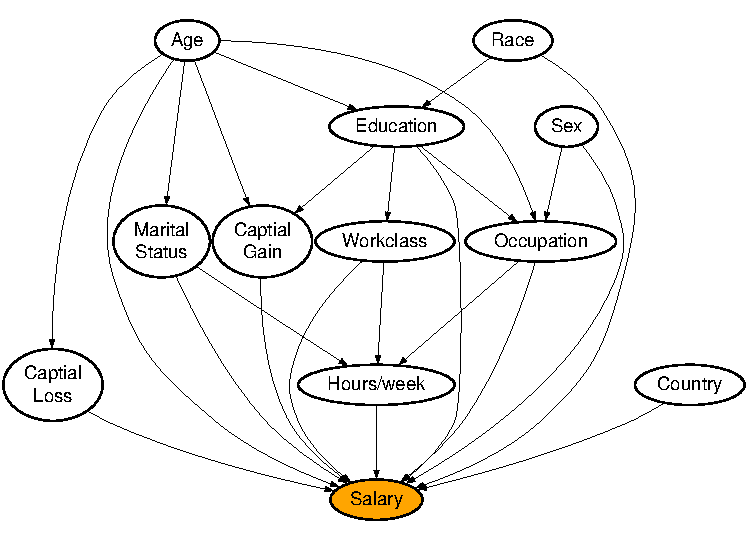
\includegraphics[width=\linewidth]{figures/graph/reference.pdf}
        \caption{Reference Graph}
        \label{fig:structure_groundtruth}
    \end{subfigure}%
    \hfill 
    \begin{subfigure}[b]{0.3\textwidth}
        \centering
        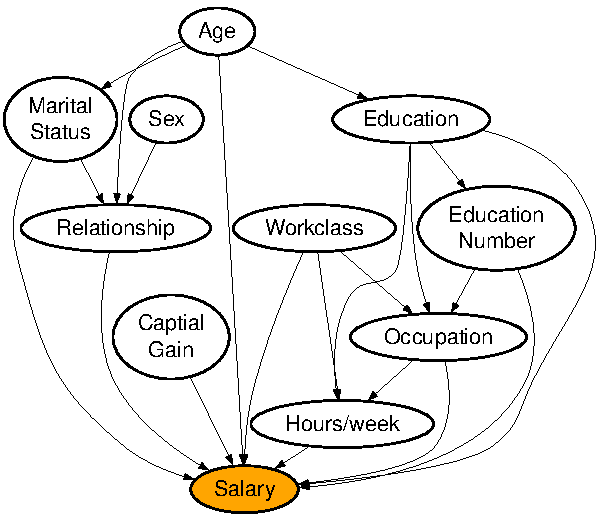
\includegraphics[width=\linewidth]{figures/graph/llm.pdf}
        \caption{LLM-Discovered}
        \label{fig:structure_llmcd}
    \end{subfigure}%
    \hfill 
    \begin{subfigure}[b]{0.32\textwidth}
        \centering
        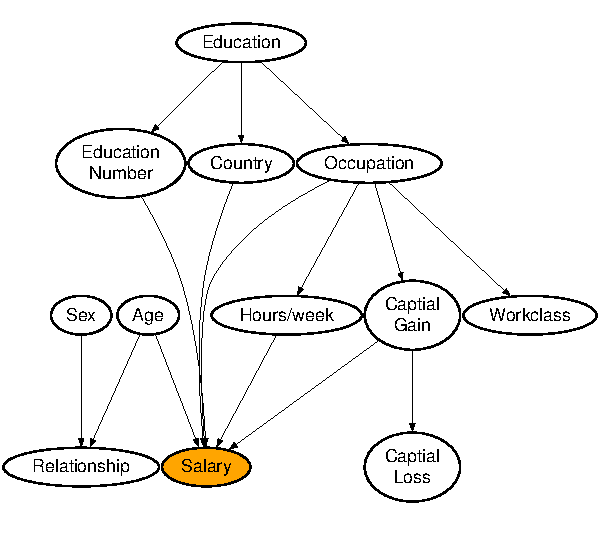
\includegraphics[width=\linewidth]{figures/graph/structsynth.pdf}
        \caption{Re-discovered from Synthetic Data}
        \label{fig:structure_structsynth}
    \end{subfigure}
    \caption{Visual Analysis of Structural Fidelity on the Adult Dataset with \textit{Salary} as the Label Column.}
    \label{fig:structure}
\end{figure*}

\subsection{Structure Discovery Comparisons on Asia Dataset}
\label{app:structure_examples}
To provide a concrete illustration of the structural discovery capabilities discussed above, Figure~\ref{fig:structure_examples} presents a visual comparison of the dependency graphs learned by \textsf{StructSynth} and four representative baselines on the Asia dataset ($n=100$). Although the Asia benchmark is defined as a causal Bayesian network, StructSynth uses the ground-truth DAG only as a reference directed dependency structure for SHD evaluation. The \textbf{Ground Truth} graph represents the reference dependency structure of the dataset, where, for example, \textit{smoke} is linked to \textit{lung} (cancer) and \textit{bronc} (bronchitis), which in turn are linked to \textit{dysp} (dyspnoea).

\textsf{StructSynth} successfully recovers the majority of these key dependencies, including the V-structure at \textit{dysp} and the dependency chain from \textit{smoke} to \textit{lung}. The slight deviations are minimal and do not disrupt the global topological ordering, ensuring that the subsequent generation process follows a valid dependency path.

In contrast, baseline methods exhibit significant structural distortions:
\begin{itemize}[leftmargin=*]
    \item \textbf{GraDe} tends to produce an overly dense graph with numerous spurious edges (e.g., direct links between \textit{asia} and \textit{dysp}), likely due to its reliance on attention maps that can conflate indirect associations with direct dependencies.
    \item \textbf{GOGGLE}, while capturing some dependencies, suffers from edge reversals (e.g., \textit{lung} $\rightarrow$ \textit{smoke}) and misses critical connections (e.g., \textit{bronc} is isolated from \textit{dysp}). This reflects the instability of end-to-end differentiable structure learning in low-data regimes.
    \item \textbf{NoTears} yields a sparse and fragmented graph, failing to identify the relationship between \textit{smoke} and \textit{lung}, which are central to the dataset's dependency structure.
    \item \textbf{FCI}, a constraint-based method, correctly identifies some skeletons but leaves many edges undirected (represented by bi-directed or unoriented edges), failing to provide a clear generative order.
\end{itemize}

These visual examples corroborate our quantitative findings in Figure~\ref{fig:shd}, confirming that \textsf{StructSynth}'s LLM-guided approach offers superior robustness in discovering interpretable and accurate dependency structures compared to both traditional and deep learning-based alternatives.

\begin{figure*}[t!]
\centering
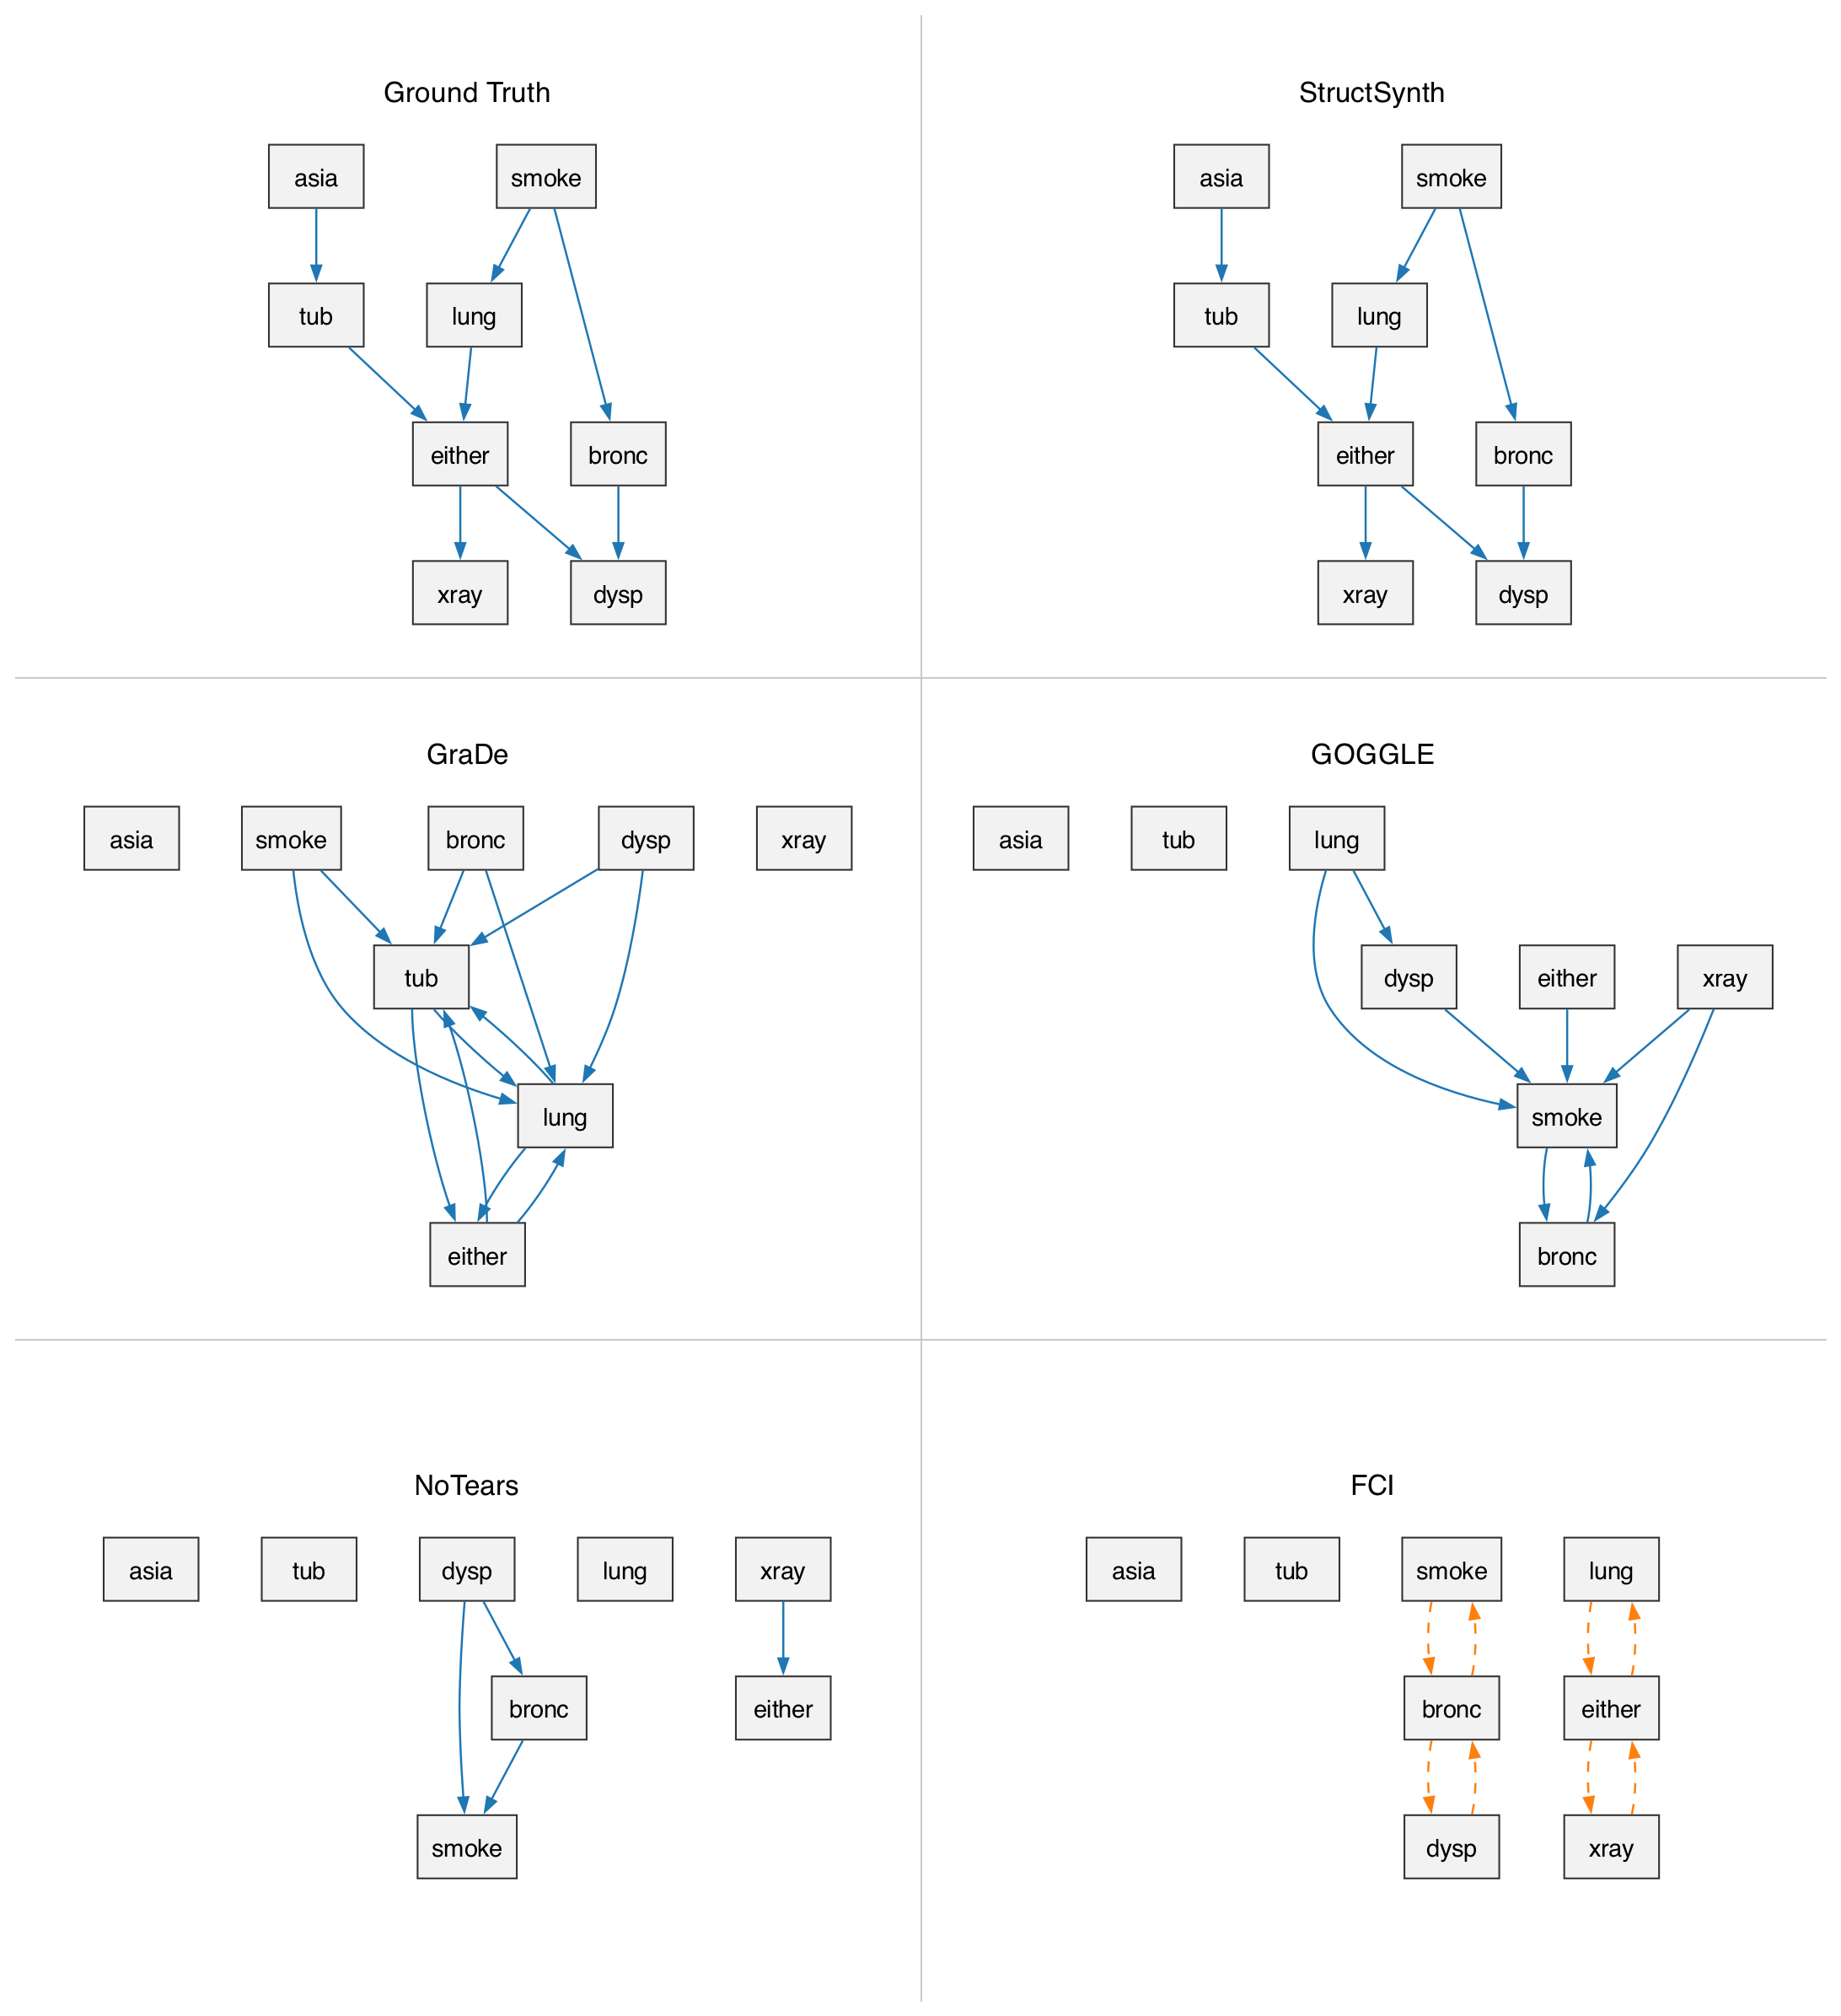
\includegraphics[width=\textwidth]{figures/collage_3x2.png}
\caption{Comparison of discovered dependency structures on the Asia dataset ($n=100$). \textbf{Ground Truth}: The reference DAG from the bnlearn repository. \textbf{StructSynth}: Our method closely recovers the ground truth. \textbf{GraDe, GOGGLE, NoTears, FCI}: Baseline methods exhibit varying degrees of structural errors, including missing edges, reversed edges, and spurious connections.}
\label{fig:structure_examples}
\end{figure*}

\section{Sensitivity to Downstream Model Choice}
\label{app:downstream_sensitivity}

To verify that the gains reported in the main experiments are not specific to a single evaluation model, we compare \textsf{StructSynth} and CLLM under four downstream learners---XGBoost (tree-based), Random Forest (ensemble), Logistic Regression / Ridge (linear), and MLP (neural)---on four representative datasets spanning classification, regression, and post-cutoff settings (Table~\ref{tab:downstream_sensitivity}). \textsf{StructSynth} wins 14 out of 16 cells, outperforming both CLLM and the train-only baseline across all three classification datasets under every evaluation model. The two exceptions occur on the Salary regression task, where Ridge and MLP favor $\mathcal{D}_\mathtt{train}$ and CLLM respectively, suggesting that linear and shallow neural models are more sensitive to distributional shifts in regression settings. Across classification datasets, the margin is largest for MLP (+3.26 AUC on Adult), indicating that neural models benefit most from the improved distributional quality of StructSynth's synthetic data.

\begin{table}[h]
\small
\centering
\caption{Downstream performance (\%) with different evaluation models on four representative datasets. (C): AUC, (R): $R^2$. Best per cell in \textbf{bold}.}
\setlength{\tabcolsep}{0.9mm}
\begin{tabular}{ll|ccc}
    \hline
    \textbf{Dataset} & \textbf{Eval.\ Model} & $\mathcal{D}_\mathtt{train}$ & \textbf{CLLM} & \textbf{StructSynth} \\
    \hline
    \multirow{4}{*}{\makecell[l]{Adult\\(C)}}
    & XGBoost & $82.51$ & $83.95$ & $\boldsymbol{85.55}$ \\
    & Random Forest & $85.03$ & $84.63$ & $\boldsymbol{87.45}$ \\
    & Logistic Reg. & $85.68$ & $85.49$ & $\boldsymbol{87.80}$ \\
    & MLP & $83.63$ & $83.59$ & $\boldsymbol{86.85}$ \\
    \hline
    \multirow{4}{*}{\makecell[l]{Anxiety$^\dag$\\(C)}}
    & XGBoost & $85.49$ & $85.17$ & $\boldsymbol{86.45}$ \\
    & Random Forest & $86.85$ & $85.14$ & $\boldsymbol{87.04}$ \\
    & Logistic Reg. & $87.26$ & $85.87$ & $\boldsymbol{87.82}$ \\
    & MLP & $84.85$ & $82.27$ & $\boldsymbol{85.76}$ \\
    \hline
    \multirow{4}{*}{\makecell[l]{Salary$^\dag$\\(R)}}
    & XGBoost & $49.71$ & $54.53$ & $\boldsymbol{55.98}$ \\
    & Random Forest & $55.16$ & $51.29$ & $\boldsymbol{57.12}$ \\
    & Ridge & $\boldsymbol{59.48}$ & $52.58$ & $56.80$ \\
    & MLP & $44.61$ & $\boldsymbol{46.00}$ & $42.64$ \\
    \hline
    \multirow{4}{*}{\makecell[l]{Churn\\(C)}}
    & XGBoost & $86.86$ & $89.81$ & $\boldsymbol{90.39}$ \\
    & Random Forest & $90.78$ & $91.66$ & $\boldsymbol{92.49}$ \\
    & Logistic Reg. & $90.61$ & $91.91$ & $\boldsymbol{92.19}$ \\
    & MLP & $91.71$ & $92.36$ & $\boldsymbol{93.61}$ \\
    \hline
\end{tabular}
\label{tab:downstream_sensitivity}
\end{table}

\section{Efficiency Analysis}
\label{sec:token_usage}

A practical concern is the additional cost introduced by structure discovery. Table~\ref{tab:token_usage} reports the token consumption of \textsc{CLLM} and \textsf{StructSynth} under the \textbf{100-shot} setting, averaged over six real-world datasets. Overall, introducing the graph-based structure modeling in \textsf{StructSynth} does \emph{not} lead to a prohibitive cost increase: the average total usage rises from \textbf{219.8K} tokens (\textsc{CLLM} total) to \textbf{287.9K} tokens (\textsf{StructSynth} combined total), corresponding to an absolute overhead of \textbf{+68.1K} tokens (about \textbf{+31.0\%}). This overhead is relatively stable across datasets (roughly \textbf{+19\%} to \textbf{+42\%} in total), suggesting that the additional structure reasoning introduces a consistent but moderate computational budget.

A key observation is that the overhead is \textbf{highly skewed toward the input side}. Concretely, \textsf{StructSynth} increases average \emph{input} tokens by \textbf{+65.1K} (\textbf{+57.1\%}), while the \emph{output} tokens only increase by \textbf{+2.9K} (\textbf{+2.7\%}). This pattern is expected: \textsf{StructSynth} needs additional prompt context to (i) elicit and refine the dependency graph and (ii) condition the synthesis stage on the discovered structure, whereas the corresponding model responses (e.g., edge lists / compact graph representations) are short and the final table synthesis outputs remain comparable in length to \textsc{CLLM}.

Importantly, this ``input-dominant'' overhead implies that the \textbf{real monetary overhead is often smaller than what the raw total-token increase might suggest}, because in many pricing schemes output tokens are priced higher than input tokens. Taken together, the token analysis indicates that \textsf{StructSynth} achieves structure-aware generation with a \textbf{modest and practically manageable} cost increase, largely attributable to additional prompting rather than longer model generations.

\begin{table*}[t]
  \centering
  \caption{Token usage under 100-shot ($\times 10^3$ tokens). We report input/output tokens for \textsc{CLLM} and \textsf{StructSynth}; overhead compares \textsf{StructSynth} combined totals (graph+table) against \textsc{CLLM} totals.}
  \label{tab:token_usage}

  \resizebox{\textwidth}{!}{%
  \small
  \renewcommand{\arraystretch}{1.12}
  \begin{tabular}{@{}ll *{7}{S[table-format=+3.1]}@{}}
    \toprule
    \textbf{Method} & \textbf{Component} & {\textbf{Adult}} & {\textbf{Anxiety}} & {\textbf{Churn}} & {\textbf{Compas}} & {\textbf{Obesity}} & {\textbf{Salary}} & {\textbf{Avg.}} \\
    \midrule
    \multirow{3}{*}{\textsc{CLLM}}
      & Input  &  40.6 & 142.2 &  38.3 &  26.5 &  70.7 & 366.1 & 114.1 \\
      & Output & 105.2 & 175.2 & 102.6 &  79.5 &  13.5 & 158.6 & 105.8 \\
      & {\bfseries Total}
               & {\bfseries 145.8} & {\bfseries 317.4} & {\bfseries 140.9} & {\bfseries 106.0}
               & {\bfseries  84.2} & {\bfseries 524.7} & {\bfseries 219.8} \\
    \midrule
    \multirow{7}{*}{\textsf{StructSynth}}
      & Graph Input  & 38.1 &  89.0 & 41.4 & 17.1 & 43.5 & 111.1 & 56.7 \\
      & Graph Output &  1.5 &   3.1 &  2.2 &  1.0 &  1.7 &   3.1 &  2.1 \\
      \rowcolor{SubtotalGray}
      & Graph total  & 39.6 &  92.1 & 43.6 & 18.1 & 45.3 & 114.3 & 58.8 \\
      \cmidrule(lr){2-9}
      & Table Input  &  52.7 & 168.3 &  46.0 &  32.3 &  61.1 & 374.3 & 122.5 \\
      & Table Output & 114.3 & 177.4 & 102.7 &  75.9 &  12.0 & 157.1 & 106.6 \\
      \rowcolor{SubtotalGray}
      & Table total  & 167.0 & 345.7 & 148.7 & 108.2 &  73.2 & 531.4 & 229.0 \\
      \cmidrule(lr){2-9}
      & {\bfseries Combined total}
                   & {\bfseries 206.6} & {\bfseries 437.8} & {\bfseries 192.3} & {\bfseries 126.3}
                   & {\bfseries 118.4} & {\bfseries 645.7} & {\bfseries 287.9} \\
    \midrule
    \multicolumn{9}{@{}l}{\textbf{Token overhead of \textsf{StructSynth} vs. \textsc{CLLM} (Combined $-$ Total)}} \\
      & $\Delta$ Input (K)  &  50.2 & 115.1 &  49.1 &  22.9 &  33.9 & 119.3 &  65.1 \\
      & $\Delta$ Output (K) &  10.6 &   5.3 &   2.3 &  -2.6 &   0.2 &   1.6 &   2.9 \\
      & $\Delta$ Total (K)  &  60.8 & 120.4 &  51.4 &  20.3 &  34.2 & 121.0 &  68.1 \\
      \cmidrule(lr){2-9}
      & Relative Input (\%)  & 123.6 &  80.9 & 128.2 &  86.4 &  48.0 &  32.6 &  57.1 \\
      & Relative Output (\%) &  10.1 &   3.0 &   2.2 &  -3.3 &   1.5 &   1.0 &   2.7 \\
      & Relative Total (\%)  &  41.7 &  37.9 &  36.5 &  19.2 &  40.6 &  23.1 &  31.0 \\
    \bottomrule
  \end{tabular}}%
\end{table*}

\section{Extended Discussion}
\label{app:extended_discussion}

In this section, we discuss the broader implications of our results, analyze key design decisions, and contextualize StructSynth within the landscape of structure-aware generative methods.

\subsection{Structure-Blind vs.\ Structure-Aware Generation}
\label{sec:structure_discussion}
A central question raised by our work is whether explicit structural guidance provides a \emph{qualitative}---rather than merely quantitative---advantage over structure-blind LLM generation. To address this, we compare StructSynth against its closest structure-blind counterpart, CLLM, which uses the same LLM with identical hyperparameters but generates data without any structural generation plan.

Our ablation study (Table~\ref{tab:ablation_study}) provides direct evidence for three distinct dimensions of improvement. First, regarding \textbf{structural modeling}: CLLM processes features in an arbitrary serialized order, implicitly inducing dependencies from the input sequence. In contrast, StructSynth encodes dependencies as an explicit DAG, ensuring that relationships are \emph{discovered} rather than incidentally induced. Second, regarding \textbf{generation strategy}: CLLM generates all features in a single pass without constraints, whereas StructSynth follows a topological ordering so that each feature is conditioned on its discovered parent nodes. Removing this ordering alone (\textit{No Topological Order} variant) degrades AUC by 1.1 points, while removing the graph entirely (\textit{No Structure} variant, equivalent to CLLM) causes a 1.6-point drop. Third, regarding \textbf{regularization}: the DAG serves as a structural regularizer that constrains the generation space, preventing the LLM from overfitting to spurious patterns in the few available training samples. This regularization effect is evidenced by StructSynth's superior privacy preservation (avg.\ rank 1.50 vs.\ CLLM's 3.50), indicating reduced memorization of training records.

These results demonstrate that the advantage of StructSynth is \emph{not} merely the result of adding peripheral components to an LLM pipeline, but stems from a fundamental shift in how dependencies are modeled and enforced during generation.

\subsection{Understanding the Fidelity-Privacy Trade-off}
\label{sec:fidelity_discussion}
A nuanced finding in our evaluation is that StructSynth does not achieve the highest Statistical Fidelity score (avg.\ rank 8.50), despite its strong downstream utility (avg.\ rank 1.00) and privacy preservation (avg.\ rank 1.50). We argue that this apparent discrepancy is both expected and desirable, reflecting the inherent tension between fidelity and privacy.

To understand this trade-off, consider GReaT, which achieves strong Statistical Fidelity (avg.\ rank 4.00). However, its Privacy Risk score of 90.15\% reveals severe memorization---the model essentially reproduces training records rather than generating novel samples. This high fidelity is therefore an artifact of overfitting rather than genuine distributional learning. At the other extreme, the Bayesian Sampler in our ablation achieves the best raw fidelity score (48.86) but the lowest AUC (81.17), conclusively demonstrating that \textbf{high pairwise fidelity does not guarantee downstream utility}.

This discrepancy can be further understood by examining what Statistical Fidelity actually measures. The metric quantifies the preservation of \emph{pairwise} correlations across all feature pairs. In contrast, StructSynth's DAG encodes \emph{conditional} dependencies---the probabilistic relationships between parent and child nodes. These conditional dependencies are what drive downstream model performance, as they capture the generative mechanisms underlying the data. StructSynth optimizes for preserving these conditional structures rather than pairwise statistics, which explains its superior utility despite moderate pairwise fidelity scores.

In summary, StructSynth's generation plan acts as a \emph{principled regularizer}: it constrains the generation process to follow discovered conditional dependencies, which simultaneously prevents memorization (ensuring privacy) and preserves the dependency structure that matters most for downstream tasks (ensuring utility), even at the cost of slightly lower pairwise correlation matching.

\subsection{When Does Structural Guidance Help Most?}
\label{sec:when_helps}
Our experiments on varying training sample sizes (Figure~\ref{fig:influence_n}) reveal that StructSynth's advantage is most pronounced in the low-data regime ($n \leq 50$), where it maintains high AUC while baselines deteriorate significantly. As $n$ increases toward 200, the performance gap narrows, though StructSynth remains competitive.

This pattern has an intuitive explanation. When data is scarce, statistical methods for structure discovery (e.g., PC algorithm, NoTears) suffer from unstable association estimates, leading to unreliable graphs. In this regime, StructSynth's LLM-guided discovery provides a powerful complement: the model's semantic prior knowledge acts as a \emph{structural regularizer}, stabilizing the discovery process by filtering out statistically spurious correlations that would mislead purely data-driven approaches. As more data becomes available, statistical methods become increasingly reliable on their own, diminishing the relative advantage of LLM-guided reasoning.

This analysis also reveals StructSynth's natural boundary conditions. The method is best suited for scenarios where: (1) the number of training samples is severely limited ($n \leq 100$); (2) features have semantically meaningful names and relationships that an LLM can reason about; and (3) the underlying dependency structure is sparse enough to be well-represented by a DAG. In contrast, for purely numerical datasets with opaque feature names (e.g., anonymized sensor readings), the LLM's semantic prior provides less value, and the framework may offer diminished advantages over purely statistical approaches.

\subsection{Relationship to Causal Inference}
It is important to clearly distinguish StructSynth's dependency graphs from causal graphs in the traditional sense. As established in Appendix~\ref{sec:why_dag}, our DAG serves as a \emph{generative dependency structure}---its edges encode statistical and probabilistic dependencies used to organize the synthesis process, not claims of ground-truth causality.

This distinction separates StructSynth from classical causal discovery methods such as the PC algorithm~\cite{spirtes2000causation}, FCI~\cite{spirtes2000causation}, or GES~\cite{chickering2002optimal}, which aim to identify the true causal data-generating mechanism under specific assumptions (e.g., faithfulness, sufficiency). Our objective is fundamentally different: we seek a dependency structure that enables \emph{effective conditional generation}, not one that supports causal interventions or counterfactual reasoning.

Nevertheless, our SHD evaluations on benchmark DAGs (Figure~\ref{fig:shd}) demonstrate that the structures discovered by StructSynth often closely approximate the ground-truth causal graphs. This is not a contradiction: when the true data-generating process follows a DAG, a well-discovered dependency structure will naturally align with the causal structure, even though causal identification is not our explicit goal. This alignment is a desirable side effect that contributes to the high fidelity of our generated data.

\section{Detailed Prompts for StructSynth}
\label{app:prompts}
This section provides a guide to the prompt templates used in the StructSynth framework. A key step in our methodology is the textualization of diverse data structures---including statistical scores, dependency graphs, and tabular data---to serve as inputs for the Large Language Model (LLM). \hyperref[box:textualization_examples]{Box 1} shows concrete examples of this process. 

The StructSynth pipeline employs a sequence of prompts to complete its tasks. First, the \hyperref[prompt:source]{\texttt{$\pi_\mathtt{source}$}} prompt initiates graph discovery by identifying initial root nodes. During the iterative graph construction, the \hyperref[prompt:generation]{\texttt{$\pi_\mathtt{generate}$}} prompt proposes new dependency edges with corresponding rationales. If a cycle is detected, the \hyperref[prompt:resolve]{\texttt{$\pi_\mathtt{resolve}$}} prompt is used to analyze the conflict and remove the weakest link. Finally, for data synthesis, the \hyperref[prompt:data_gen]{\texttt{$\pi_\mathtt{data\_gen}$}} prompt generates values for dependent features, after which the \hyperref[prompt:data_gen_iso]{\texttt{$\pi_\mathtt{iso}$}} prompt generates values for the remaining isolated features.


\begin{tcolorbox}[
    float*=t, width=\textwidth, floatplacement=htbp,
    colback=teal!10!white,  % Light teal background
    colframe=teal!60!black, % Dark teal frame
    title={Examples of Data Textualization for LLM Prompts}, % Box title
    fonttitle=\bfseries\color{white}, % Title font bold, color white
    arc=2mm, % rounded corners
    boxrule=1pt % thickness of the frame
] 

\small % Use a smaller font size for the content within the box

\textbf{1. Textual Representation of Statistical Evidence (Association Scores):}
\begin{verbatim}
Association scores for 'Education', scaled 0 to 1.
(Levels: >0.8 Very High, >0.6 High, >0.4 Moderate, >0.2 Low, <=0.2 Very Low)

- Occupation: 0.85 (Very High)
- Salary: 0.72 (High)
- Marital-Status: 0.55 (Moderate)
- Hours-per-week: 0.31 (Low)
- Sex: 0.12 (Very Low)
\end{verbatim}

\vspace{\medskipamount} % Add space

\textbf{2. Textual Representation of a Dependency Graph:}
\begin{verbatim}
Current dependency graph structure with rationales:
- Age -> Marital-Status
Rational: A person's age is a primary factor influencing their marital status.

- Sex -> Relationship: 
Rational: Gender often determines the relationship role within a household.

- Country -> Race: 
Rational: Native country has a strong statistical correlation with a person's race.

- Race -> Education: 
Rational: Statistical data often shows a correlation between a person's race 
and their level of educational attainment.

\end{verbatim}

\vspace{\medskipamount} % Add space

\textbf{3. Textual Representation of Tabular Data (Markdown):}
\begin{verbatim}
| age | education   | occupation      | sex    | hours-per-week | salary |
|-----|-------------|-----------------|--------|----------------|--------|
| 39  | Bachelors   | Adm-clerical    | Male   | 40             | <=50K  |
| 50  | Bachelors   | Exec-managerial | Male   | 13             | <=50K  |
| 28  | Assoc-acdm  | Prof-specialty  | Female | 45             | <=50K  |
\end{verbatim}
\label{box:textualization_examples}
\end{tcolorbox}




\begin{tcolorbox}[
    float*=t, width=\textwidth, floatplacement=htbp,
    colback=yellow!10!white,  % Light yellow background
    colframe=yellow!75!black, % Dark gold/ochre frame
    title={Prompt for Source Nodes Initialization of Tabular Data ($\pi_\mathtt{source}$)}, % Box title
    fonttitle=\bfseries\color{white}, % Title font bold, color black 
    arc=2mm, % rounded corners
    boxrule=1pt % thickness of the frame
]
\small % Use a smaller font size for the content within the box

You are an expert data analyst. Based on the following information:

\vspace{\medskipamount}

\textbf{Task Description:}

Identify the initial "source nodes" for a dependency graph. A source node is a root attribute that is generated without conditioning on other attributes in this dataset.


\vspace{\medskipamount}

\textbf{All Feature Descriptions:}
\begin{verbatim}
{all_features}
\end{verbatim}

\vspace{\medskipamount}

\textbf{Example Data:}
\begin{verbatim}
{few_shot_data}
\end{verbatim}

\vspace{\medskipamount}

\textbf{Your Task is to Identify the Source Nodes:}
\begin{itemize}[leftmargin=*, itemsep=2pt]
    \item Your only task is to analyze the provided column descriptions and data.
    \item Identify the features that are most likely to be \textbf{source nodes} (i.e., fundamental attributes that are not dependent on other features).
    \item Provide your answer as a simple list of the identified source node names.
\end{itemize}
\label{prompt:source}
\end{tcolorbox}



\begin{tcolorbox}[
    float*=t, width=\textwidth, floatplacement=htbp,
    colback=pink!10!white,  % Light pink background
    colframe=pink!75!black, % Dark pink/magenta frame
    title={Prompt for Link Generation in Dependency Discovery ($\pi_\mathtt{generate}$)}, % Box title
    fonttitle=\bfseries\color{white}, 
    arc=2mm, % rounded corners
    boxrule=1pt % thickness of the frame
]
\small % Use a smaller font size for the content within the box

You are an expert data analyst building a dependency graph. Based on the following information:

\vspace{\medskipamount} % Add space

\textbf{Task Description:}

For the given $\texttt{\{current\_feature}\}$, your task is to propose its direct successors (dependents) 
from the list of available features. For each proposed dependency, you must provide a 
brief, evidence-based rationale.

\vspace{\medskipamount} % Add space

\textbf{Current Graph State:}
\begin{verbatim}
{structure_graph}
\end{verbatim}
\vspace{\medskipamount} % Add space

\textbf{All Candidate Features:}
\begin{verbatim}
{all_features}
\end{verbatim}
\vspace{\medskipamount} % Add space

\textbf{Statistical Evidence (Association Scores):}
\begin{verbatim}
{association_scores}
\end{verbatim}
\vspace{\medskipamount} % Add space

\textbf{Example Data:}
\begin{verbatim}
{few_shot_data}
\end{verbatim}
\vspace{\medskipamount} % Add space

\textbf{Your Task is to Propose and Justify New Links:}
\begin{itemize}[leftmargin=*, itemsep=2pt]
    \item Your focus is on the feature: $\texttt{\{current\_feature}\}$.
    \item Review the \textbf{Statistical Evidence}, which shows the strength of association between $\texttt{\{current\_feature\}}$ and other candidate features $\texttt{\{all\_features\}}$.
    \item Based on the statistical scores, the example data, and the existing graph, identify which other features are most likely to be \textbf{direct dependents} of $\texttt{\{current\_feature\}}$.
    \item For each dependency you propose, you \textbf{must} provide a concise $\texttt{rationale}$. This rationale should explain why the dependency makes sense (e.g., "Higher Education is strongly correlated with and typically precedes higher Income").
    \item Do not propose links that would create an obvious logical contradiction with the existing graph structure.
    \item Format your final output as a list of dependency edges and their corresponding rationales.
\end{itemize}

\label{prompt:generation}
\end{tcolorbox}

\begin{tcolorbox}[
    float*=t, width=\textwidth, floatplacement=htbp,
    colback=green!10!white,  % Light green background
    colframe=green!60!black, % Dark green frame
    title={Prompt for Cycle Resolution in Dependency Discovery ($\pi_\mathtt{resolve}$)}, % Box title
    fonttitle=\bfseries\color{white}, % Title font bold, color white
    arc=2mm, % rounded corners
    boxrule=1pt % thickness of the frame
]
\small % Use a smaller font size for the content within the box

You are a logical reasoning expert tasked with resolving a contradiction in a dependency graph. Based on the following information:

\vspace{\medskipamount} % Add space

\textbf{Task Description:}

Analyze the provided dependencies and their rationales within the cycle. Identify the 
single dependency with the weakest or least plausible rationale and recommend it for 
removal to break the cycle.

\vspace{\medskipamount} % Add space

\textbf{Conflicting Cycle with Rationales:}
\begin{verbatim}
{cycle_with_rationales}
\end{verbatim}
\vspace{\medskipamount} 

\textbf{Your Task is to Identify the Weakest Link:}
\begin{itemize}[leftmargin=*, itemsep=2pt]
    \item A logical contradiction (a cycle) has been detected in the graph, detailed in \textbf{Conflicting Cycle with Rationales}.
    \item Your task is to carefully evaluate the \texttt{rationale} provided for each edge in this cycle.
    \item Based on your analysis of the rationales and any relevant context from the column descriptions or data, identify the \textbf{single weakest link}.
    \item The weakest link is the dependency whose rationale is the least plausible, least supported, or most likely to be spurious.
    \item Provide your final answer as the single dependency edge that should be removed to resolve the contradiction.
\end{itemize}

\label{prompt:resolve}
\end{tcolorbox}

\begin{tcolorbox}[
    float*=t, width=\textwidth, floatplacement=htbp,
    colback=blue!5!white,  % Light blue background
    colframe=blue!75!black, % Dark blue frame
    title={Prompt for Graph-Planned Conditional Synthesis ($\pi_\mathtt{data\_gen}$)}, % Box title
    fonttitle=\bfseries\color{white}, % Title font bold, color white
    arc=2mm, % rounded corners
    boxrule=1pt % thickness of the frame
]
\small 

You are a helpful AI assistant that generates realistic tabular data based on structural dependencies.

\vspace{\medskipamount} % Add space

\textbf{Task Description:}

Generate a realistic synthetic table containing exactly the columns listed in 
$\texttt{\{features\_to\_generate\}}$. This generation must be conditioned on the provided values 
of their parent features.

\vspace{\medskipamount} % Add space

\textbf{Conditioning Data (Current Results):}
\begin{verbatim}
{current_result}
\end{verbatim}
\vspace{\medskipamount} % Add space

\textbf{Relevant Dependency Structure:}
\begin{verbatim}
{related_structure_graph}
\end{verbatim}
\vspace{\medskipamount} % Add space

\textbf{Example Data:}
\begin{verbatim}
{related_few_shot_data}
\end{verbatim}
\vspace{\medskipamount} % Add space

\textbf{Your Task is to Generate the Synthetic Data:}
\begin{itemize}[leftmargin=*, itemsep=2pt]
    \item Your primary task is to generate realistic data for the features listed in $\texttt{\{features\_to\_generate\}}$.
    \item This generation must be \textbf{conditioned} on the data provided in \textbf{Conditioning Data (Current Results)}. These are the values of the parent nodes that influence the features you are generating.
    \item The \textbf{Relevant Dependency Structure} shows you exactly how the conditioning features relate to the features you need to generate.
    \item Use the \textbf{Example Data} to understand the format, range, and statistical properties of the real data.
    \item The generated table should contain columns for exactly the features listed in $\texttt{\{features\_to\_generate\}}$.
    \item Ensure the generated values are plausible and respect the learned dependencies.
\end{itemize}

\label{prompt:data_gen}
\end{tcolorbox}

\begin{tcolorbox}[
    float*=t, width=\textwidth, floatplacement=htbp,
    colback=purple!10!white,  % Light purple background
    colframe=purple!75!black, % Dark purple frame
    title={Prompt for Independent Feature Synthesis ($\pi_\mathtt{iso}$)}, % Box title
    fonttitle=\bfseries\color{white}, % Title font bold, color white
    arc=2mm, % rounded corners
    boxrule=1pt % thickness of the frame
]
\small % Use a smaller font size for the content within the box

You are a helpful AI assistant that completes tabular data records by generating values for remaining features.

\vspace{\medskipamount} % Add space

\textbf{Task Description:}

The core, structurally-dependent features of a dataset have already been generated. 
Your task is to generate plausible values for the remaining isolated features, ensuring they are statistically consistent with the core features.

\vspace{\medskipamount} % Add space

\textbf{Conditioning Data (Generated Graph-Based Features):}
\begin{verbatim}
{graph_based_values}
\end{verbatim}
\vspace{\medskipamount} % Add space

\textbf{Features to Generate (Isolated Features):}
\begin{verbatim}
{isolated_features_to_generate}
\end{verbatim}
\vspace{\medskipamount} % Add space

\textbf{Example Data:}
\begin{verbatim}
{related_few_shot_data}
\end{verbatim}
\vspace{\medskipamount} % Add space

\textbf{Your Task is to Generate the Independent Values:}
\begin{itemize}[leftmargin=*, itemsep=2pt]
    \item Your primary task is to generate realistic data for the features listed in $\texttt{\{isolated\_features\_to\_generate}\}$.
    \item This generation must be \textbf{conditioned} on the complete set of core features provided in \textbf{Conditioning Data}.
    \item The features you are generating do not have direct parent-child dependencies in the learned graph, but their values should still be plausible and consistent in the context of the entire data record.
    \item Use the \textbf{Example Data} to understand the typical format and statistical properties of these isolated features.
    \item The generated table should contain columns for exactly the features listed in $\texttt{\{isolated\_features\_to\_generate}\}$.
\end{itemize}
\label{prompt:data_gen_iso}
\end{tcolorbox}

\clearpage
